% Assignment 1 - Neurorobotics 2025/2026 - LORANDI Enzo
% Compile: pdflatex main.tex  (run twice for references)
% Layout per the assignment: max 12 pages, double column,
% margins top 1.5 cm, bottom 1.3 cm, inner/outer 1.5 cm.

\documentclass[10pt,twocolumn,a4paper]{article}

\usepackage[top=1.5cm,bottom=1.3cm,left=1.5cm,right=1.5cm]{geometry}
\usepackage[utf8]{inputenc}
\usepackage[T1]{fontenc}
\usepackage{amsmath}
\usepackage{graphicx}
\usepackage{booktabs}
\usepackage{caption}
\usepackage{subcaption}
\usepackage[hidelinks]{hyperref}

\graphicspath{{../figures/}}

\usepackage{tikz}
\usetikzlibrary{arrows.meta,positioning}

\usepackage{titlesec}
\titleformat{\section}{\large\bfseries}{\thesection}{0.6em}{}[{\titlerule[0.8pt]}]
\titlespacing*{\section}{0pt}{1.1em}{0.5em}

\begin{document}

% ---- Title block spanning both columns ----
\twocolumn[
  \begin{center}
    {\LARGE\bfseries Motor-Imagery BCI Decoding:\\[2pt]
     Grand Average and a Subject-Specific Control Framework\par}
    \vspace{0.6em}
    {\large LORANDI Enzo\par}
    \vspace{0.2em}
    {\itshape Neurorobotics 2025/2026, University of Padova\par}
    \vspace{1.0em}
  \end{center}
]

% =====================================================
\section{Introduction}
\label{sec:intro}

A brain--computer interface (BCI) lets a person control a device using only
brain activity, without any real movement. In this work the brain signals are
EEG, and the person performs \emph{motor imagery} (MI): they only
\emph{imagine} a movement. Here the two tasks are imagining both hands moving or
both feet moving. The system reads the EEG and must guess which task the person
is doing.

The EEG (electroencephalogram) is a non-invasive technique that records the
electrical activity of the brain with electrodes placed on the scalp. The
measured signal does not come from a single neuron: one neuron is far too small
to be seen from outside the head. The EEG is the \emph{sum} of the activity of a
large population of cortical neurons (mainly pyramidal cells) that are active at
the same time. Because the signal must cross the brain, the skull and the skin,
it is very small (about 10--100\,$\mu$V) and noisy, so it needs careful
processing before it can be used.

The brain produces rhythms (oscillations) at different frequencies. I focus on
the \emph{mu} band (about 8--12\,Hz) and the \emph{beta} band (about
18--30\,Hz), which are linked to movement. When many neurons in the motor area
work in synchrony, the power of these rhythms is high; when the person imagines
a movement, the neurons desynchronize and the power goes down. This decrease is
called event-related desynchronization (ERD), and the return increase is
event-related synchronization (ERS). Imagining the hands and imagining the feet
involve slightly different parts of the motor cortex, so the power change is not
in the same place: this is what lets me tell the two tasks apart. Motor imagery
is a \emph{self-paced} activity (there is no fixed external stimulus and the
response is different in each trial), so I describe it with the power in
frequency bands over time rather than with the average signal shape.

The goal of this assignment is to analyse an MI dataset recorded from eight
people over three days. The work has two parts. First, a \emph{grand average}
over all subjects, to find which features carry the most useful information (a
feature is one channel at one frequency). Second, a \emph{decoding} part for
each subject: I train a classifier on the calibration (offline) runs, test it
on the online runs, and then add a \emph{control framework} that adds up the
evidence over time. This last step turns many noisy guesses (one per time
window) into a single, more reliable decision for each trial.

This analysis was not written from zero. During the course labs (Lab~02 to
Lab~09) I built and tested small reusable MATLAB functions, step by step. Each
lab added one block of the pipeline: reading the data, filtering, band power,
the spectrogram, the features, the classifier, and finally the control
framework. In this assignment I reuse these functions
(Section~\ref{sec:pipeline}) and apply the same pipeline to every subject.
Building the pipeline one lab at a time, and then writing it here, helped me
understand how each step connects to the next.

% =====================================================
\section{Materials and Methods}

\begin{figure*}[t]
\centering
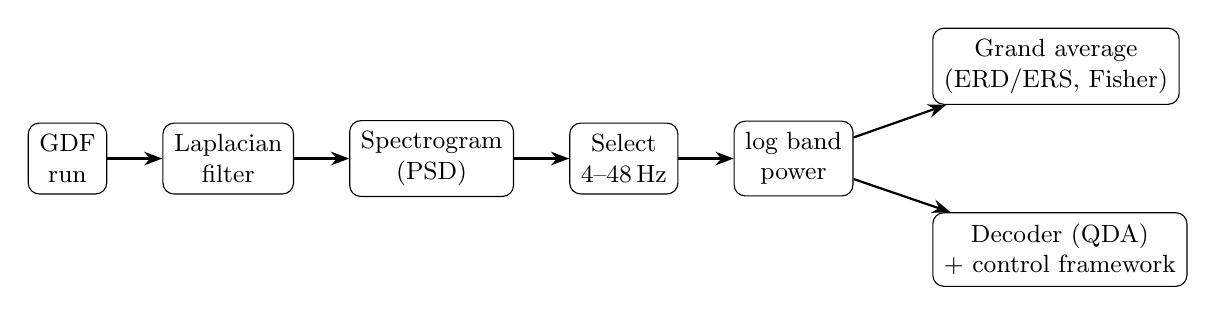
\begin{tikzpicture}[
  box/.style={draw, rounded corners, align=center, inner sep=4pt,
              minimum height=9mm, font=\small},
  arr/.style={-{Stealth}, thick}]
\node[box] (a) {GDF\\run};
\node[box, right=7mm of a] (b) {Laplacian\\filter};
\node[box, right=7mm of b] (c) {Spectrogram\\(PSD)};
\node[box, right=7mm of c] (d) {Select\\4--48\,Hz};
\node[box, right=7mm of d] (e) {log band\\power};
\node[box, above right=2mm and 10mm of e] (f) {Grand average\\(ERD/ERS, Fisher)};
\node[box, below right=2mm and 10mm of e] (g) {Decoder (QDA)\\+ control framework};
\foreach \x/\y in {a/b,b/c,c/d,d/e} \draw[arr] (\x)--(\y);
\draw[arr] (e)--(f);
\draw[arr] (e)--(g);
\end{tikzpicture}
\caption{Overview of the pipeline. The same processing (Laplacian, spectrogram,
frequency selection, log band power) is applied to every run; the resulting
features feed both the grand average and the per-subject decoder with its
control framework.}
\label{fig:pipeline}
\end{figure*}

\subsection{From the labs to a reusable toolbox}
\label{sec:pipeline}

One important choice in this work is that the analysis was not written as one big
script. Instead, the pipeline is split into small reusable functions (called
utilities) that are kept together in a single MATLAB folder. Each function does
one clear job, such as loading a file, applying a filter, or computing the
features. A lab script then only describes the scientific steps and calls these
functions. This keeps the code short, easy to read, and easy to reuse.
Figure~\ref{fig:pipeline} gives an overview of the whole pipeline.

These utilities were not written all at once. They were built and tested step by
step during the course labs, and Table~\ref{tab:labs} shows which lab produced
which function. Labs 02 and 03 handle reading the GDF files, joining several runs
together, and building the label vectors. Lab 04 adds the band power. Lab 05 adds
the spatial filters (CAR and Laplacian). Labs 06 and 07 move to a time and
frequency representation (ERD/ERS and the spectrogram). Lab 08 adds the feature
selection with the Fisher score, and Lab 09 adds the control framework. Because
each function was already tested on a single subject during its lab, I could
trust it and reuse it directly for the eight subjects of this assignment.

Two functions, \texttt{proc\_spectrogram} and \texttt{proc\_pos2win}, were
provided by the course (CNBI toolbox), while all the other utilities were written
by me. For this assignment I also added a few small helpers, for example one to
load and join the processed files of a subject and one to build the per-window
labels, so that the analysis scripts stay short and the same code is shared by
every subject.

The project itself is organised to keep three things separate: the reusable
functions, the lab experiments, and the assignment. The reusable functions are
in \texttt{matlab/utils}. Each lab has its own folder under
\texttt{matlab/labs}, with its script, a short README, and its figures. The
assignment is in \texttt{assignments/assignment1}, which holds the analysis
scripts (\texttt{scripts}), the figures of this report (\texttt{figures}), and
the report (\texttt{report}). The EEG data is stored in a separate \texttt{data}
folder (raw, external, and processed) and, following the submission rules, it is
not included in the deliverable.

\begin{table}[h]
\centering
\caption{Utilities introduced across the labs and reused in this assignment
($\dagger$~provided by the course, all others written by the author).}
\label{tab:labs}
\small
\begin{tabular}{@{}lp{2.0cm}p{3.1cm}@{}}
\toprule
Lab & Topic & Utility produced \\
\midrule
02, 03 & GDF I/O, concatenation & \texttt{load\_gdf\_file}, \texttt{concat\_gdf\_runs}, \texttt{create\_label\_vectors} \\
04     & Log band power & \texttt{compute\_bandpower} \\
05     & Spatial filters & \texttt{apply\_car\_filter}, \texttt{apply\_laplacian\_filter} \\
06, 07 & ERD/ERS, spectrogram & \texttt{proc\_spectrogram}$^{\dagger}$, \texttt{proc\_pos2win}$^{\dagger}$ \\
08     & Feature selection & \texttt{compute\_fisher\_score} \\
09     & Control framework & \texttt{apply\_control\_framework} \\
\bottomrule
\end{tabular}
\end{table}

\subsection{Dataset and paradigm}
\label{sec:data}

The dataset comes from a motor-imagery experiment with eight subjects (named
ai6 to aj9). The EEG was recorded with a 16-channel g.USBamp amplifier at
512\,Hz, and the electrodes were placed following the 10--20 system. Each
subject was recorded on more than one day. For every subject there are three
offline runs and several online runs spread over the days. The offline runs are
the calibration runs: the feedback always moves in the correct direction, so
this clean data is used for the grand average and to train the decoder. The
online runs are the evaluation runs: the feedback is driven by the classifier,
so they show how the system works in real use, and they are kept only for
testing.

Each run is a sequence of trials. A trial begins with a fixation cross, then a
cue tells the subject which movement to imagine (both hands or both feet), and
finally a continuous feedback period follows. These moments are marked in the
recording by event codes: 786 for the fixation cross, 771 for both feet, 773 for
both hands, and 781 for the continuous feedback. I use these codes to cut the
signal into trials and to know the true class of each trial. In this work the
decoding is a two-class problem between both hands and both feet.

\subsection{Signal processing and features}
\label{sec:proc}

Before computing the features, the EEG is cleaned and transformed in the same
way for every run. First, a Laplacian spatial filter is applied. For each
channel it subtracts a weighted average of its neighbours, which removes the
activity shared by many channels and keeps the local activity over the motor
cortex. This makes the motor-imagery patterns easier to see than on the raw
channels.

Next, the power of the signal is computed over time and frequency. I use the
provided function \texttt{proc\_spectrogram}, which estimates the power spectral
density (PSD) in short sliding windows. The main parameters are listed in Table~\ref{tab:spec}. The output gives one
value for each time window, each
frequency, and each channel. With a 512\,Hz sampling rate, this gives a
frequency step of 2\,Hz and one window every 0.0625\,s (about 16 windows per
second).

\begin{table}[h]
\centering
\caption{Spectrogram parameters used in \texttt{proc\_spectrogram}.}
\label{tab:spec}
\small
\begin{tabular}{@{}lr@{}}
\toprule
Parameter & Value \\
\midrule
Outer window length & 0.5\,s \\
Outer window step   & 0.0625\,s \\
Inner (PSD) step    & 0.25\,s \\
Moving average      & 1\,s \\
\bottomrule
\end{tabular}
\end{table}

From the full PSD I keep only the frequencies from 4 to 48\,Hz, with a step of
2\,Hz (23 frequencies). This range covers the mu and beta rhythms that are
useful for motor imagery, and it removes the very low and very high frequencies
that carry little information or more noise.

Finally, I take the logarithm of the band power. The log makes the values more
symmetric and closer to a normal distribution, which helps the later steps (the
Fisher score and the classifier) work better. A feature is therefore the log
power of one channel at one frequency.

Because the spectrogram changes the time axis from samples to windows, the event
positions and durations also have to be converted from samples to windows. This
is done with the provided function \texttt{proc\_pos2win}, so that the events
still point to the correct moments in the new representation.

\subsection{Grand-average ERD/ERS}
\label{sec:erd}
To see where and when the motor-imagery activity appears, I compute the ERD/ERS
on the offline runs. For each trial I use two periods: the fixation period as the
reference (the brain before the cue) and the continuous feedback period as the
activity. The ERD/ERS compares the band power during the activity with the band
power during the reference, so a negative value means the power went down (ERD)
and a positive value means it went up (ERS). I compute this comparison in
decibels (dB), as a log ratio between the activity power $A$ and the reference
power $R$ (Eq.~\ref{eq:erd}).

\begin{equation}
\label{eq:erd}
\mathrm{ERD/ERS} = 10\,\log_{10}\!\frac{A}{R},
\qquad R = \overline{P_{\text{fixation}}} .
\end{equation}

At first I used the usual percentage form, $100\,(A-R)/R$, but it gave
unrealistic values: on a few channels the reference power was very small, so
dividing by it produced huge numbers (several thousand percent) that hid the real
pattern. The dB form is bounded and symmetric, it is not sensitive to a
near-zero reference, and it is consistent with the log power features used in the
rest of the pipeline. For these reasons I report the ERD/ERS in dB.

The ERD/ERS is first averaged over the trials of each class, for each subject, in
the mu and beta bands. To obtain a result for the whole population, these
per-subject maps are then averaged across the eight subjects. The population maps
are shown as scalp topographies in the Results (Section~\ref{sec:res-ga}), and
they let me check that the activity appears over the expected motor areas.

\subsection{Feature selection (Fisher score)}
\label{sec:fisher}
After the processing, each time window is described by 16 channels times 23
frequencies, which gives 368 features (one log power value per channel and
frequency). Most of these features are not useful for telling the two tasks
apart, so I need a way to find the best ones.

For this I use the Fisher score. For each feature, it compares the two classes:
it is large when the means of the two classes are far apart and the values inside
each class are not too spread out (Eq.~\ref{eq:fisher}).

\begin{equation}
\label{eq:fisher}
F_k = \frac{\big(\mu_k^{(1)}-\mu_k^{(2)}\big)^2}
           {\big(\sigma_k^{(1)}\big)^2 + \big(\sigma_k^{(2)}\big)^2} .
\end{equation}

A high Fisher score means the feature separates both hands and both feet well. I
compute the Fisher score on the continuous-feedback windows of the offline runs,
where the subject is actually performing the task.

I then select the features with the highest Fisher score (here the best two).
Using only a few strong features keeps the classifier simple and avoids the
problems that appear when there are too many features for the number of trials.

\subsection{Classification}
\label{sec:clf}

With the selected features, I train a classifier that learns to separate the two
classes. I use a discriminant analysis classifier (the MATLAB function
\texttt{fitcdiscr}) with a quadratic boundary (QDA). A quadratic boundary lets
each class have its own shape in the feature space, which fits the data better
than a single straight line when the two clouds of points have different spreads.

The classifier is trained only on the offline runs, using the
continuous-feedback windows (the task period). For each new window the trained
model gives two things: the predicted class (both hands or both feet) and the
posterior probabilities, which say how confident the model is for each class.
These probabilities are important, because the control framework
(Section~\ref{sec:control}) will use them, and not only the final class.

\subsection{Control framework: evidence accumulation}
\label{sec:control}

A single window gives a noisy decision, so using only one window would not be
reliable. The control framework solves this by adding up the evidence over time.
At each window it mixes the new posterior probability with the value from the
previous window, using an exponential smoothing (Eq.~\ref{eq:control}). The
parameter $\alpha$ controls the memory: a value close to 1 gives a slow and
smooth curve, which is more stable but slower to react.

\begin{equation}
\label{eq:control}
D(t) = \alpha\,D(t-1) + (1-\alpha)\,p(t),
\qquad D(\text{trial start}) = 0.5 .
\end{equation}

The accumulated value $D$ is reset to 0.5 at the start of every trial, so each
trial begins with no evidence for either class. A decision is made for the trial
when $D$ reaches a fixed threshold (here 0.2 for one class and 0.8 for the
other). The moment when the threshold is reached also gives the time to deliver
the command. If $D$ never reaches a threshold during the trial, the trial can be
rejected (no command is sent), which trades fewer commands for a higher accuracy
on the trials that are kept.

\subsection{Evaluation metrics}
\label{sec:metrics}

I evaluate the decoder with three measures. The single-sample accuracy is the
percentage of windows that are classified correctly during the
continuous-feedback period. The trial accuracy is the percentage of trials for
which the control framework gives the correct decision; I report it both without
rejection (every trial gets a decision) and with rejection (trials that never
reach a threshold are removed). The third measure is the average time to deliver
a command, that is the mean time from the trial start to the moment the threshold
is reached.

I also separate offline and online performance. For the offline (calibration)
runs I use a 5-fold cross-validation for the single-sample accuracy, because
training and testing on the very same data would give a result that is too
optimistic. The online (evaluation) runs are kept apart and are never used for
training, so they give an honest measure of the real performance. For the offline
trial accuracy I apply the trained decoder to its own offline data
(resubstitution); this value is therefore optimistic and is used only as a
reference, while the online numbers are the meaningful ones.

% =====================================================
\section{Results}

\subsection{Grand average and most relevant features}
\label{sec:res-ga}

Figure~\ref{fig:fisher} shows the population Fisher map, averaged over the eight
subjects. The most discriminative features are over the hand motor area, on
channel C3 around 12 to 14\,Hz (in the mu and low-beta range). This matches what
is expected for hand versus feet motor imagery, and it confirms that the pipeline
finds meaningful features automatically.

Figure~\ref{fig:topo} shows the population ERD/ERS topographies (in dB) during
the activity period, for the mu and beta bands and for both classes. For both
hands, the power decreases (ERD) over the lateral central area (C3 and C4), which
are the hand regions. For both feet, the change is weaker and more central
(around Cz, the foot region), with a relative increase (ERS) over the hand area.
The mu band shows a stronger and clearer pattern than the beta band.

The subjects are not all the same. Using the peak Fisher score as a simple
measure of how separable the two classes are, subject aj1 is the most
discriminable and subject aj7 is the least (close to chance). This large
difference between subjects is a known effect in motor-imagery BCI, where some
users produce clear sensorimotor changes and others do not.

\begin{figure}[h]
  \centering
  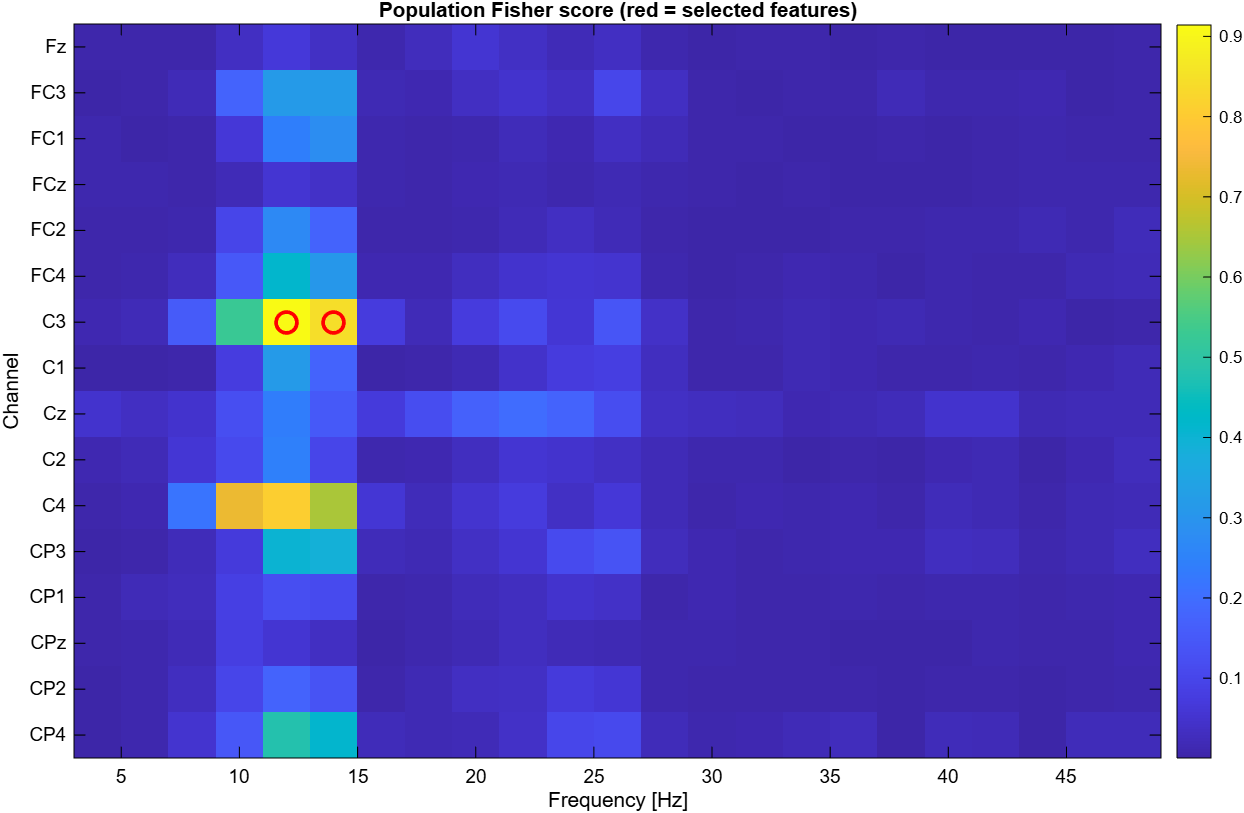
\includegraphics[width=\columnwidth]{grandavg_fisher_map.png}
  \caption{Population-averaged Fisher score for every channel-frequency
  feature (red circles: selected features).}
  \label{fig:fisher}
\end{figure}

\begin{figure}[h]
  \centering
  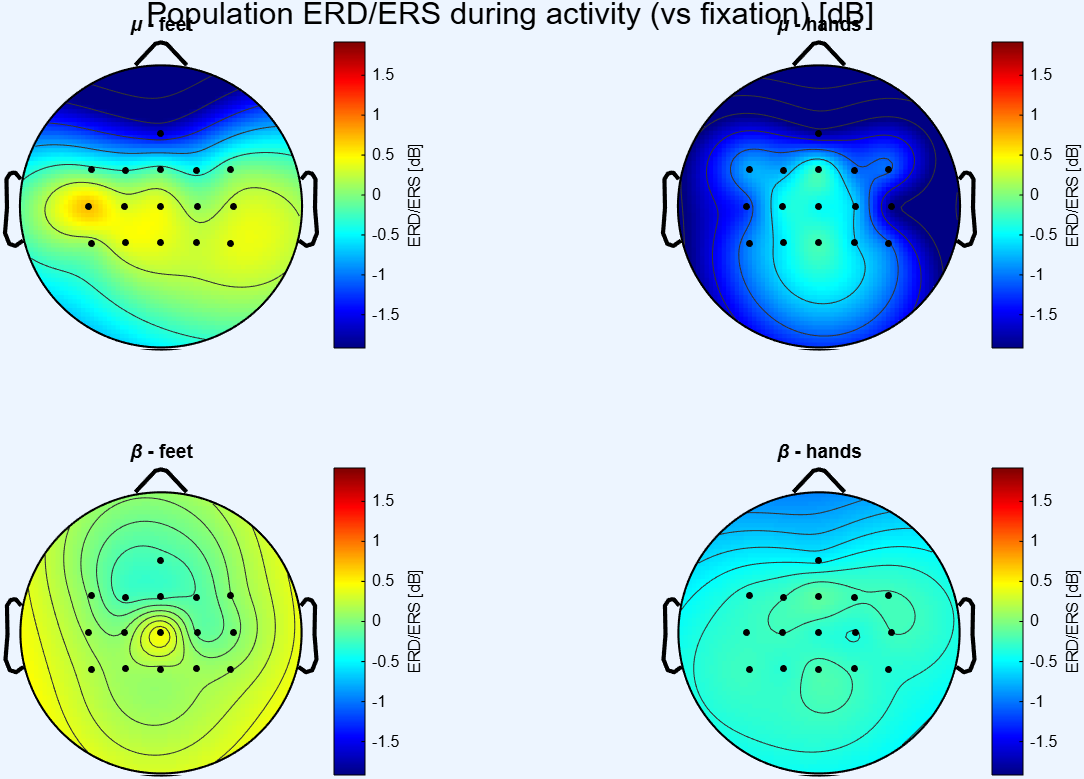
\includegraphics[width=\columnwidth]{grandavg_erd_topographies.png}
  \caption{Population ERD/ERS (dB) during the activity period, $\mu$ and
  $\beta$ bands, both classes.}
  \label{fig:topo}
\end{figure}

\subsection{Calibration (offline)}
\label{sec:res-cal}

Table~\ref{tab:calib} reports, for each subject, the two selected features and
the offline single-sample accuracy measured by 5-fold cross-validation. The mean
accuracy over the eight subjects is 84.6\,\%, which is good for a two-class
problem that uses only two features. The selected features are almost always over
the sensorimotor channels (C3, C4, C1, Cz, CP3, CP4) in the mu and low-beta
range, and they are different from one subject to another. This is why the
decoder is trained for each subject separately. The results also follow the grand
average: subject aj1 reaches 94.7\,\% while subject aj7 stays at 69.0\,\%, close
to chance.

\begin{table}[h]
\centering
\caption{Offline calibration per subject: selected features and 5-fold
cross-validation single-sample accuracy (features given as channel@frequency,
in Hz).}
\label{tab:calib}
\small
\begin{tabular}{@{}llr@{}}
\toprule
Subject & Selected features & CV acc.\,(\%) \\
\midrule
ai6 & Cz@20, Cz@18   & 77.9 \\
ai7 & C4@14, C3@14   & 90.2 \\
ai8 & C3@14, C4@14   & 87.5 \\
aj1 & C4@10, C4@12   & 94.7 \\
aj3 & C3@14, C3@12   & 88.5 \\
aj4 & C1@12, C3@12   & 80.7 \\
aj7 & CP4@10, C4@12  & 69.0 \\
aj9 & CP4@12, CP3@12 & 88.0 \\
\midrule
Mean &              & 84.6 \\
\bottomrule
\end{tabular}
\end{table}

\subsection{Online evaluation}
\label{sec:res-eval}

Figure~\ref{fig:evidence} shows the control framework on one trial of subject
aj1. The raw probability of a single window is noisy, but the integrated evidence
rises smoothly and reaches the threshold, which delivers the correct command.
This is the behaviour I want from the accumulation step.

Figure~\ref{fig:ss} compares the single-sample accuracy offline and online for
each subject. The online accuracy is lower than the offline one (mean
76.2\,\% online against 84.6\,\% offline). This drop is expected, because the
online runs are recorded on different days and use real feedback, so the signal
is harder to classify.

Figure~\ref{fig:trial} shows the trial accuracy with rejection, and
Figure~\ref{fig:time} shows the average time to deliver a command. Even though the
single-sample accuracy is only 76.2\,\% online, the trial accuracy reaches
90.7\,\% on average (88.9\,\% without rejection). This large gain is the main
benefit of the control framework: by adding up many windows, it removes most of
the single-window errors and gives a reliable decision per trial. The average
time to deliver a command is about 2.9\,s, and on average about 32\,\% of the
trials are rejected. This shows the usual trade-off in a BCI: a higher accuracy
can be reached, but it costs some time and some rejected trials.

\begin{figure}[h]
  \centering
  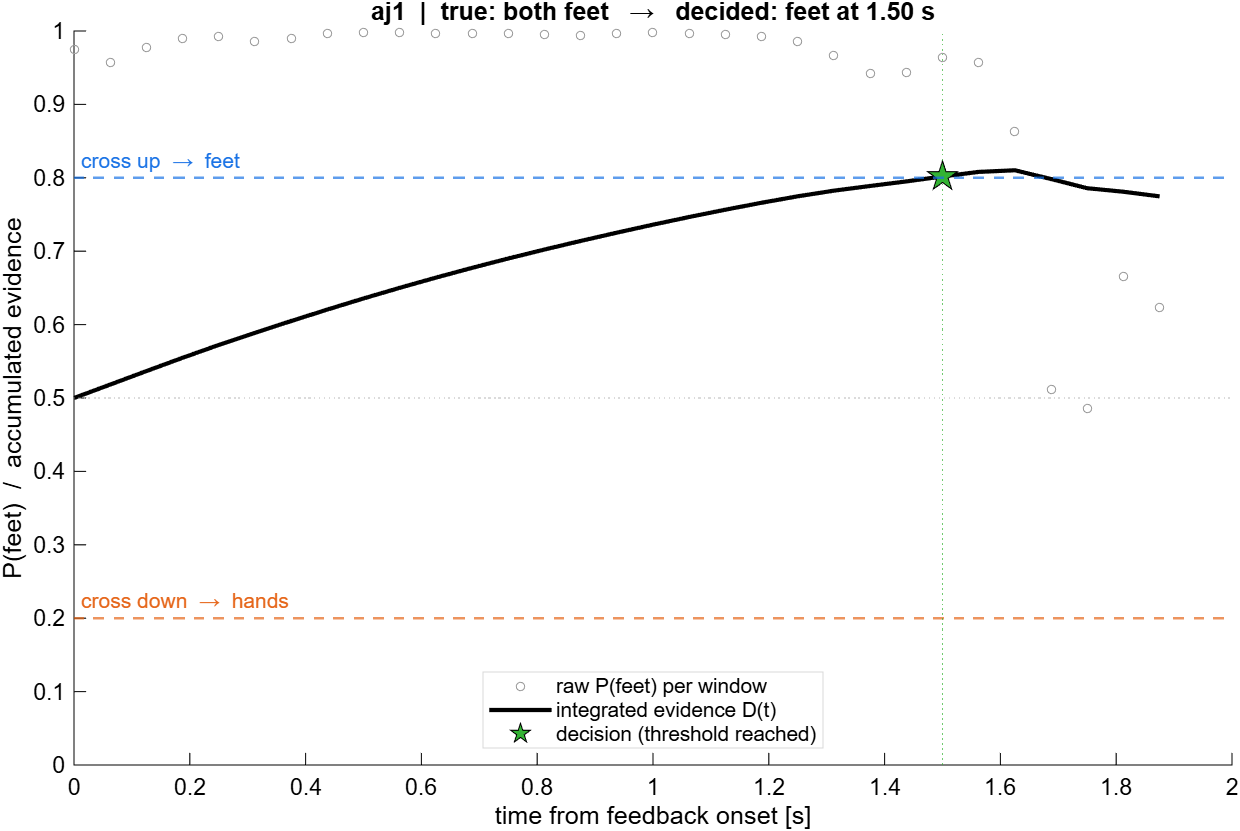
\includegraphics[width=\columnwidth]{decoding_evidence_accumulation.png}
  \caption{Evidence accumulation on a representative trial (subject aj1):
  the integrated evidence reaches the threshold and a command is delivered.}
  \label{fig:evidence}
\end{figure}

\begin{figure}[h]
  \centering
  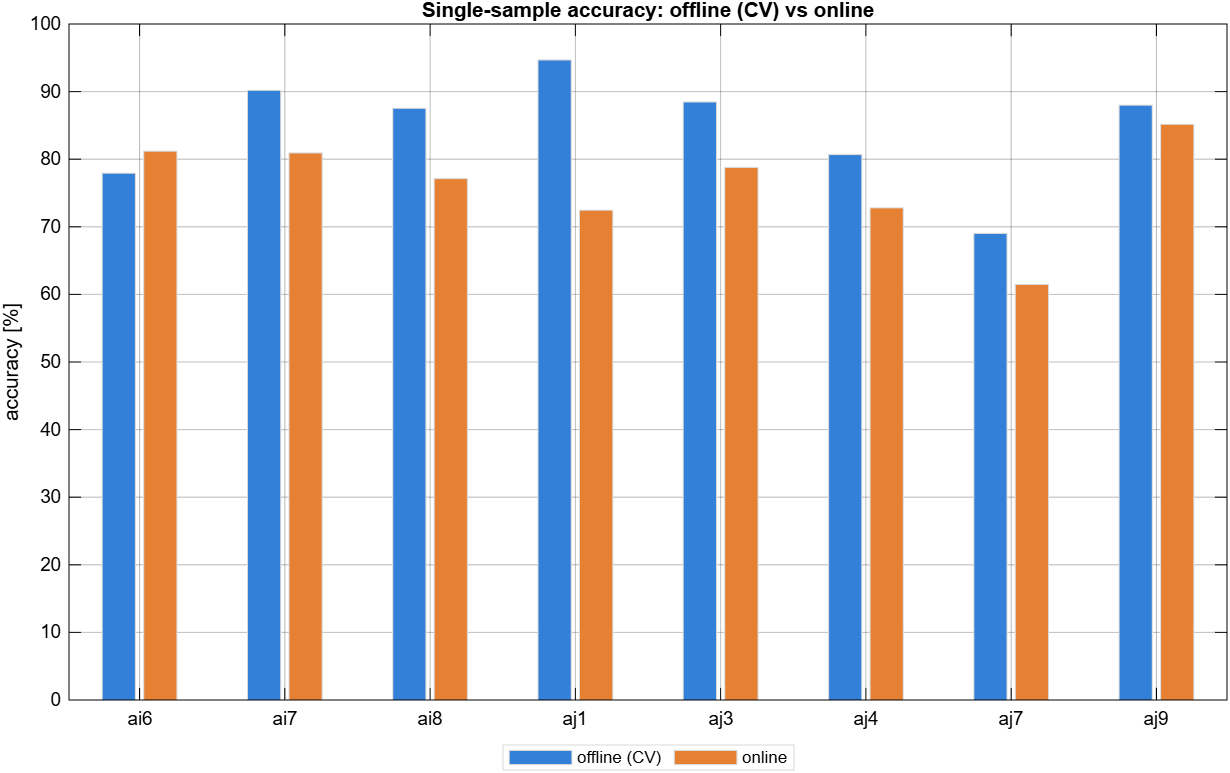
\includegraphics[width=\columnwidth]{decoding_single_sample_accuracy.png}
  \caption{Single-sample accuracy per subject: offline (5-fold CV) vs online.}
  \label{fig:ss}
\end{figure}

\begin{figure}[h]
  \centering
  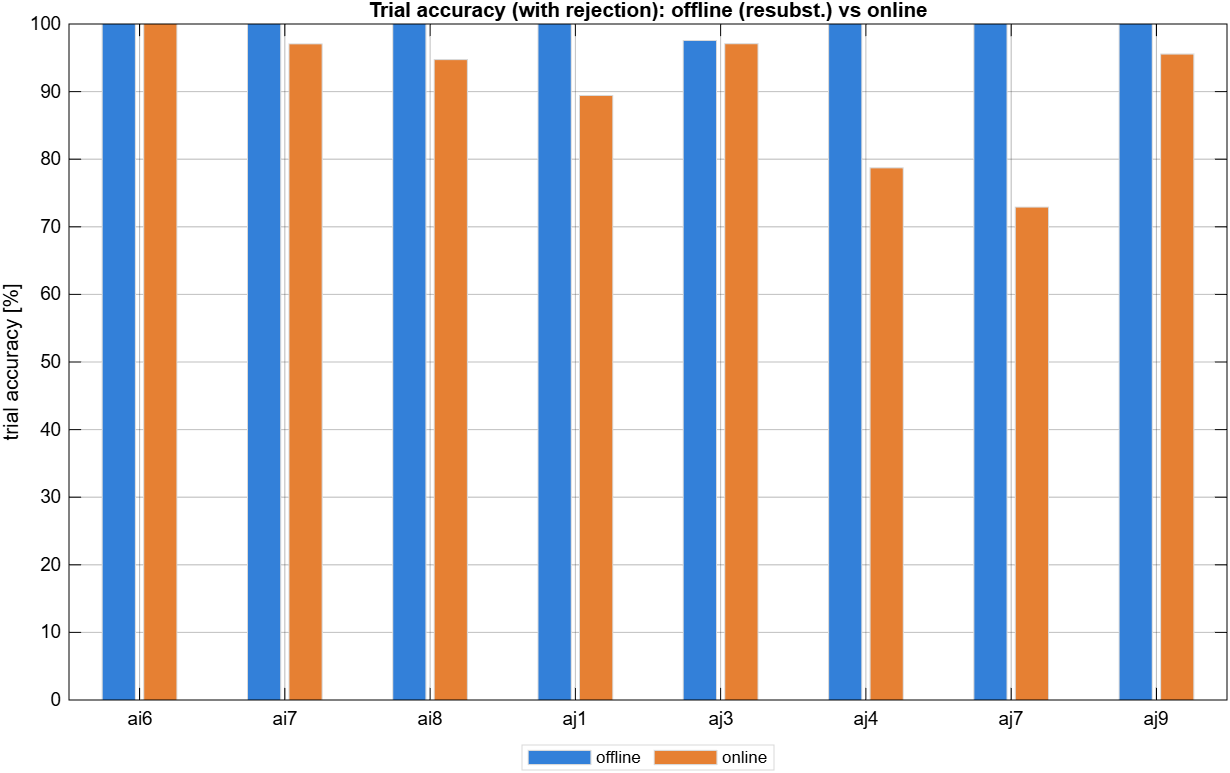
\includegraphics[width=\columnwidth]{decoding_trial_accuracy.png}
  \caption{Trial accuracy with rejection per subject: offline (resubstitution)
  vs online.}
  \label{fig:trial}
\end{figure}

\begin{figure}[h]
  \centering
  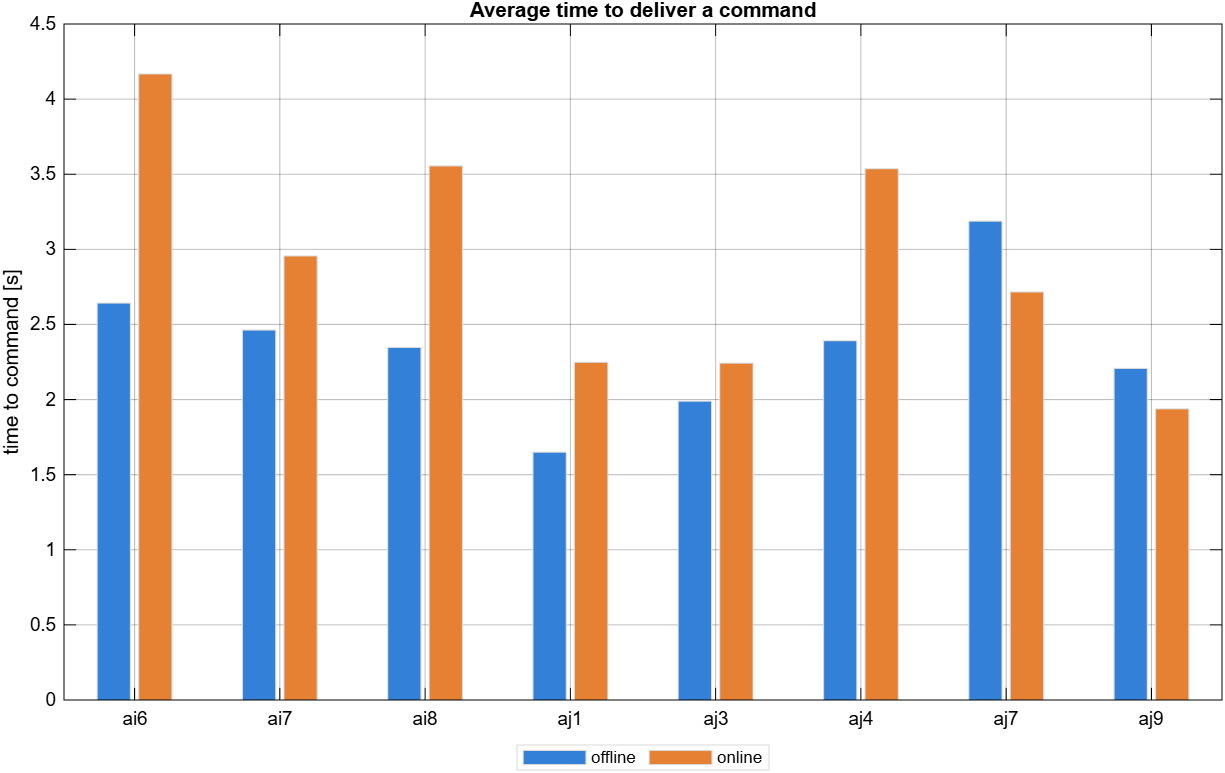
\includegraphics[width=\columnwidth]{decoding_time_to_command.png}
  \caption{Average time to deliver a command per subject.}
  \label{fig:time}
\end{figure}

% =====================================================
\section{Discussion}
\label{sec:discussion}

The results show a clear pattern. On the offline data the decoder reaches a good
single-sample accuracy (84.6\,\% on average), but on the online data this drops
to 76.2\,\%. This difference is expected: the online runs are recorded on other
days and the subject receives real feedback, so the brain signals are not exactly
the same as during calibration. A decoder trained once on the first day must
still work later, and this is harder.

The most important result is the gain given by the control framework. The
single-sample accuracy online is only 76.2\,\%, but the trial accuracy reaches
about 90\,\%. By accumulating the evidence over time, the system turns many noisy
window decisions into one reliable decision per trial. This is exactly why a
control framework is used in real BCIs, instead of trusting a single window.

The performance is not the same for every subject. Subject aj1 is good both
offline and online, while subject aj7 stays close to chance. This effect,
sometimes called BCI inefficiency, is well known: some users do not produce
strong or stable sensorimotor rhythms, and no decoder can fully fix this. It also
shows the value of training the decoder for each subject.

The framework also involves a trade-off. With rejection the trial accuracy is
higher, but some trials give no command and the average time to deliver a command
grows. The right balance between accuracy, speed and number of commands depends
on the application.

This work has some limits. I report the ERD/ERS in dB rather than in percent,
which is more robust but changes the unit. The offline trial accuracy is computed
by resubstitution, so it is optimistic and is only a reference. I use only two
features and fixed values for alpha and the thresholds; tuning these for each
subject could improve the results. These choices keep the pipeline simple and the
same for every subject, but they leave room for improvement.

% =====================================================
\section{Conclusion}
\label{sec:conclusion}

In this assignment I built a full motor-imagery BCI analysis, reusing a toolbox
that I developed step by step during the course labs. On eight subjects, the
grand average showed that the most useful features are over the hand motor area
in the mu and low-beta range. A simple decoder with two features per subject
reached 84.6\,\% single-sample accuracy offline and 76.2\,\% online. Most
importantly, the evidence-accumulation control framework raised the online
performance to about 90\,\% at the trial level, with a command delivered in about
2.9\,s. These results confirm both the difficulty of moving from calibration to
real online use, and the strong value of accumulating evidence over time to
obtain reliable commands.

% =====================================================
\begin{thebibliography}{9}
\small
\bibitem{tonin2020} L. Tonin \textit{et al.}, ``The role of the control
framework for continuous teleoperation of a BMI-driven mobile robot,''
\textit{IEEE Trans. Robot.}, vol.~36, no.~1, pp.~78--91, 2020.
\bibitem{pfurtscheller2001} G. Pfurtscheller \textit{et al.}, ``Motor imagery
and direct brain--computer communication,'' \textit{Proc. IEEE}, vol.~89,
no.~7, pp.~1123--1134, 2001.
\bibitem{wolpaw2004} J. R. Wolpaw \textit{et al.}, ``Control of a
two-dimensional movement signal by a noninvasive brain--computer interface in
humans,'' \textit{PNAS}, vol.~101, no.~51, pp.~17849--17854, 2004.
\bibitem{leeb2013} R. Leeb \textit{et al.}, ``Transferring brain--computer
interfaces beyond the laboratory: Successful application control for
motor-disabled users,'' \textit{Artif. Intell. Med.}, vol.~59, no.~2,
pp.~121--132, 2013.
\bibitem{perdikis2018} S. Perdikis \textit{et al.}, ``The Cybathlon BCI race:
Successful longitudinal mutual learning with two tetraplegic users,''
\textit{PLOS Biol.}, vol.~16, no.~5, e2003787, 2018.
\end{thebibliography}

\end{document}
